%!TEX root = ../dissertation.tex
\chapter{Modeling Aspects}
\label{chap:modeling}
\section{Continuum systems}\label{sec:continua_Model}
Matters are composed of discrete objects such as molecules, yet studying macroscopic systems down to the discrete particles is challenging. For analytic purposes in many cases, it can be assumed that matters  distributed  \textit{continuously}.  Continuum mechanics is the study of systems with such an assumption. This allows for studying the motion of macroscopic systems from fluids to solids without the need to model discrete underlying objects. The objective of the following section is to describe the fundamental principals of continua to the extent relevant in this manuscript.

\subsection{Definitions}
Throughout section \S\ref{sec:continua_Model}, the following conventions are used to denote the quantities associated with continua. \textit{Scalar} (zero-rank tensor) variables are denoted by lower or upper case light face Latin and Greek letters, e.g. $\rho$ and $\phi$. Bold face lower case Latin letters, e.g. $\vect{u}$, are used to denote \textit{vectors} (first-order tensor) quantities. Bold face upper case Latin letters as well bold face lower case Greek letters, e.g. $\vect{E}$,  and $\bm \sigma$, are used for \textit{tensor} (second-order tensors) variables. Lastly, it is assumed that the problem is 3D and scalars, vectors, and tensors are comprised of 1, 3, and 9 elements respectively. 

\subsection{Conservation Principals in continuua}
Conservation principals is an important aspect of continua as it allows studying the conserved variables such as mass, momentum, energy and as so forth.

In a given \textit{control volume} ($\mathbf{V}$) of a continuum surrounded by the control surface ($\mathbf{S}$), illustrated in Fig.~\ref{fig:CV}, a conserved value $\phi$ behaves such that :
\begin{figure}[H]
	\begin{center}
		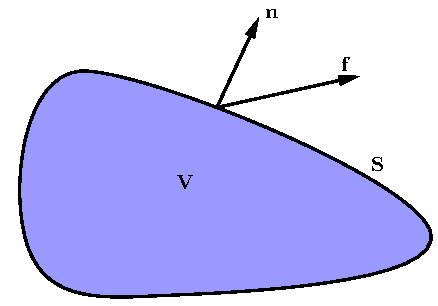
\includegraphics[width=.4\linewidth]{images/CV.pdf}
	\end{center}
	\caption{The control volume $\vect V$ bounded by the control surface $\vect S$. At every point on the control surface the vector $\vect {n}$ is pointing outward, and the $\vect{f}$ is the flux of a property that enter or exit the control volume.}
	\label{fig:CV}
\end{figure}
\begin{equation}
\parbox{4cm}{\centering the rate of change of $C$  in the control volume $\mathbf{V}$} = 
\parbox{4cm}{\centering the rate at which the $C$ enters or leave the domain through the control surface $\mathbf{S}$ } +
\parbox{4cm}{\centering the rate of generation or dissipation of $C$  inside the control volume $\mathbf{V}$}.  \label{eq:conservation}
\end{equation}
Assuming that $c=c(\vect{x},t)$ is the concentration of a scalar variable $C$ per unit mass of the control volume, $\phi(\vect{x},t)=\rho(\vect{x},t) c(\vect{x},t) $ is the concentration of $C$ per unit volume, and $\rho=\rho(\vect{x},t)$ is the density of the medium, it follows that:
\begin{equation}
C=\int_{V} c(\vect{x},t) dm= \int_{V} c(\vect{x},t) \rho(\vect{x},t) d{\vect{x}} = \int_{V} \phi (\vect{x},t) d{\vect{x}} .
\label{eq:Concentration}
\end{equation}
The flux of a variable is defined as the amount of the variable per unit area and unit time that enters or leaves ${V}$ through ${S}$. It follows from Eq.~\ref{eq:conservation} that
 \begin{equation}
\frac{\partial}{\partial t} \int_{{V}} \phi (\vect{x},t) d{\vect{x}}= 
- \int_{{S}} \vect{f}(\vect{x},t) \bigcdot \vect{n} ds+
\int_{{V}} s (\vect{x},t) d{\vect{x}},
\label{eq:conservation_integral}
\end{equation}
which is the integral form of conservation law. After applying the divergence theorem 
 \begin{equation}
\int_{{S}} \vect{f} \bigcdot \vect{n} ds=
\int_{{V}} (\nabla \bigcdot \vect{f})   d{\vect{x}},
\label{eq:divergence_theo}
\end{equation}
and assuming that the functions $\phi(\vect{x},t)$ and $\vect{f}(\vect {x},t)$ are differentiable and the divergence theorem holds, the \textit{differential form} of the conservation law is obtained as follows,
\begin{align}
\frac{\partial \phi (\vect{x},t) }{\partial t}  +
\nabla \bigcdot \vect{f}(\vect {x},t) 
-
s(\vect{x},t)=0.
\label{eq:conservation_differential}
\end{align}
The flux of $\phi$ comes from advection and diffusion of $\phi$ as follows:
\begin{align}
\vect{f}(\vect{x},t)=
\underbrace{\vect{u}(\vect{x},t) \phi(\vect{x},t)}_{\text{advection of $\phi$}} 
\underbrace{- \vect{D}(\vect{x},t) \nabla\phi(\vect{x},t)}_{\text{diffusion of $\phi$}},
\label{eq:Flux}
\end{align} 
where $\vect{D}$ is the diffusion matrix. Substituting the flux in Eq.~\ref{eq:conservation_differential} and dropping the space and time dependency for simplicity, the following general form of conservation law is obtained:
\begin{align}
\frac{\partial \phi  }{\partial t}  + \nabla \bigcdot (\vect{u} \phi - \vect{D}  \nabla \phi) -s=0
\label{eq:transport_simple}
\end{align}
%Further simplifications to the advective flux is possible assuming an incompressible flow. After incorporating the mass conservation $\nabla\bigcdot \vect{u}=0$ and using the following identity 
%\begin{align}
%\nabla \bigcdot (\vect{u}\phi)=  \vect{u} \bigcdot \nabla\phi + \phi \nabla \bigcdot \vect{u},\label{eq:identity}
%\end{align}
%the form of advection-diffusion-reaction equation of a generic transport variable $\phi$  for \textit{incompressible flow} becomes
%\begin{align}
%\frac{\partial \phi}{\partial t}  + \vect{u} \bigcdot \nabla \phi  -\nabla \bigcdot (\vect{D}  \nabla \phi) -s=0
%\label{eq:transport2}
%\end{align}
%Note that the equivalent Lagrangian form of the equation condenses the advective term and the $\frac{\partial \phi}{\partial t}$ into the material derivative as explained in Eq.~\ref{eq:Material_Derivative} as follows:
%\begin{align}
%\frac{D \phi}{Dt}   -\nabla \bigcdot (\vect{D}  \nabla \phi) -s=0
%\label{eq:transport_lagrangian}
%\end{align}


\subsection{Mass Conservation}
Assume that $c=1$, i.e. $C$ is a \textit{scalar}  specifying the concentration of mass, and the integral in Eq.~\ref{eq:Concentration} is the physical \textit{mass} of the control volume. Substituting the $\phi=\rho c=\rho$ in Eq.~\ref{eq:conservation_differential} and assuming the advective flux vector of $\vect{f}=\vect{u} \phi= \rho \vect{u} $ and no mass source ($s=0$) leads to the generic forms of the continuity equation:
\begin{subequations}
	\begin{alignat}{3}
	\frac{\partial \rho }{\partial t}  + \nabla \bigcdot (\rho \vect{u} )=0 \label{eq:continuity_1},\\
	\frac{\partial \rho }{\partial t}  +\vect{u} \bigcdot \nabla\rho + \rho \nabla \bigcdot \vect{u}=0\label{eq:continuity_2},\\
	\frac{D \rho }{D t} + \rho \nabla \bigcdot \vect{u}=0 \label{eq:continuity_3}.
	\end{alignat}\label{eq:continuity}
\end{subequations}
The last equation is derived after incorporating the material derivative, 
\begin{align}
\frac{D(\;)}{Dt}&=\frac{\partial (\;)}{\partial t} + \vect{u} \bigcdot  \nabla(\;).  \label{eq:Material_Derivative}
\end{align}
 Incompressible flow assumption ($D\rho/Dt=0$) may further simplify the mass conservation equations Eqs.~\ref{eq:continuity} to:
\begin{equation}
\nabla \bigcdot \vect{u}=0 \label{eq:continuity_incompressible}.
\end{equation}



\subsection{Momentum Conservation}
The conservation of momentum, also called Navier-Stokes equations, can be derived assuming that $c=\mathbf{u}$ and $\phi=\rho c=\rho \mathbf{u}$, i.e. $C$ is a vector specifying the momentum concentration. The flux tensor can be written as the sum of advective and stress flux, i.e. 
\begin{align}
\vect{f}=& \vect{u}(\vect{x},t) \phi(\vect{x},t) - \bm{\sigma}(\vect{x},t) =\rho\vect{u}\vect{u}-\bm\sigma \nonumber\\
=& \rho\begin{bmatrix}
u_1u_1& u_1u_2& u_1u_3\\
u_2u_1& u_2u_2& u_2u_3\\
u_3u_1& u_3u_2& u_3u_3\\
\end{bmatrix}+
\begin{bmatrix}
\sigma_{11}& \sigma_{12}& \sigma_{13}\\
\sigma_{21}& \sigma_{22}& \sigma_{23}\\
\sigma_{31}& \sigma_{32}& \sigma_{33}\\
\end{bmatrix}
\label{eq:mom_flux}
\end{align}
where $\vect{u} \vect{u}$ is a tensor results from the dyadic product of $\vect{u}$ by itself, and $\bm{\sigma}(\vect{x},t)$ is the stress flux. Substituting the flux tensor of Eq.~\ref{eq:mom_flux} in Eq.~\ref{eq:conservation_differential} results in the conservative Cauchy equations as follows
\begin{align}
\frac{\partial (\rho \vect{u})  }{\partial t}  + \nabla \bigcdot (\rho \vect{u} \vect{u} -  \bm \sigma) -s=0
\label{eq:Momentum_Eu}
\end{align}
 Further simplifications to the advective flux is possible assuming an incompressible flow. After incorporating the mass conservation $\nabla\bigcdot \vect{u}=0$ and using the following identity 
\begin{align}
\nabla \bigcdot (\vect{u}\phi)=  \vect{u} \bigcdot \nabla\phi + \phi \nabla \bigcdot \vect{u},\label{eq:identity}
\end{align}
with $\phi=\rho \vect{u}$ the second term can be simplified to 
\begin{align}
\nabla \bigcdot (\rho\vect{u}\vect{u})=\vect{u} \bigcdot \nabla(\rho\vect{u})+ \rho\vect{u} (\nabla \bigcdot \vect{u})=\vect{u} \bigcdot \nabla(\rho\vect{u}),
\end{align}
which subsequently can be used in conjunction with \ref{eq:Material_Derivative} to express the Cauchy equation in Lagrangian form as follows:
\begin{align}
\frac{ D (\rho \vect{u})  }{D t}  -\nabla \bigcdot  \bm \sigma -s=0.
\label{eq:Momentum_La}
\end{align}
Eqs.~\ref{eq:Momentum_Eu} and \ref{eq:Momentum_La} are respectively  Eulerian and Lagrangian momentum transport in any continuum. Further simplification requires more information about the nature of the continuum of interest. 
Conventionally in fluids and many other incompressible continua, $\bm{\sigma}$ can be decomposed into a volumetric (hydrostatic) part and a \textit{traceless} deviatoric part, as follows:
\begin{align}
&\bm{\sigma}=\bm{\sigma}^{dev}+\bm{\sigma}^{vol}\label{eq:stress_decomp}\\
&tr(\bm{\sigma}^{vol})=tr(\bm{\sigma})=\sigma_{11}+\sigma_{22}+\sigma_{33},\\
&tr(\bm{\sigma}^{dev})=0.
\end{align}
where $tr( )$ indicates sum of the diagonal elements of a tensor. Defining 
\begin{equation}
p=-({\sigma_{11}+\sigma_{22}+\sigma_{33}})/{3},
\end{equation}
to be the mechanical pressure, the volumetric and the deviatoric parts of the stress tensor may be written as follows:
\begin{align}
&\bm{\sigma}^{vol}=(\frac{\bm{\sigma}: \mathbf{I}}{3}) \mathbf{I}=(\frac{\sigma_{11}+\sigma_{22}+\sigma_{33}}{3}) \mathbf{I}=
-p
\begin{bmatrix}
1& 0& 0\\
0&1&0\\
0&0&1\\
\end{bmatrix},\label{eq:sigma_vol}\\
&\bm{\sigma}^{dev}=\bm{\sigma}-(\frac{\bm{\sigma}: \mathbf{I}}{3}) \mathbf{I}=
\begin{bmatrix}
\sigma_{11}& \sigma_{12}& \sigma_{13}\\
\sigma_{21}& \sigma_{22}& \sigma_{23}\\
\sigma_{31}& \sigma_{32}& \sigma_{33}\\
\end{bmatrix}+
\begin{bmatrix}
p& 0& 0\\
0&p&0\\
0&0&p\\
\end{bmatrix}.
\label{eq:sigma_dev}
\end{align}
Ultimately, substituting the flux of Eq.~\ref{eq:mom_flux}  and stress decomposition of Eqs.~\ref{eq:stress_decomp}, \ref{eq:sigma_vol} and \ref{eq:sigma_dev}  into Eq.~\ref{eq:conservation_differential} leads to:
\begin{align}
\frac{\partial \rho \vect{u} }{\partial t}  + \nabla \bigcdot (\rho\vect{u}\vect{u}-\bm{\sigma}^{vol}-\bm{\sigma}^{dev})-\vect{f}_b=0,
\label{eq:Cauchy_momentum}
\end{align}
where $\vect{f}_b$ is the body force that acts as the source term $\vect{s}$ seen in \ref{eq:conservation_differential}. According to  
\begin{align}
\nabla \bigcdot (\bm{\sigma}^{vol})=\nabla \bigcdot (p\mathbf{I})=\nabla p, 
\end{align}
the momentum conservation for Eulerian frameworks becomes:
\begin{align}
\frac{\partial (\rho \vect{u}) }{\partial t}  + \vect{u} \bigcdot \nabla(\rho\vect{u}) + \nabla p+ \nabla \bigcdot \bm{\sigma}^{dev} - \vect{f}_b=0.\label{eq:Cauchy_momentum_Eu}
\end{align}
After applying the material derivative (Eq.~\ref{eq:Material_Derivative}), the Lagrangian form of the momentum equation is obtained as follows:
 \begin{align}
 \frac{D (\rho \vect{u}) }{D t}  + \nabla p+ \nabla \bigcdot \bm{\sigma}^{dev} - \vect{f}_b=0.\label{eq:Cauchy_momentum_La}
 \end{align}
 Above, there are fewer equations than unknowns ($p, \vect{u}, \bm \sigma $) and more equations are needed to describe the material behavior. In the following section, constitutive equations required for modeling the  $\nabla \bigcdot \bm{\sigma}^{dev} $ for Newtonian and non-Newtonian fluids are described.
\subsection{Material Modeling}
\subsubsection*{Newtonian Model}
For Newtonian fluids, the deviatoric part of the stress tensor is related to the shear rate, through $\bm{\sigma}^{dev} = 2 \mu \bm E$, where $\mu$ is a constant representing the dynamic viscosity of the fluid and \textit{deformation-rate} tensor $\bm E$ is obtained from the velocity gradient tensor as follows,
\begin{align}
\bm E=\frac{1}{2}(\nabla\bf{u}+\nabla\bf{u}^T).
\label{eq:def_rate}
\end{align}
Above note that $\bm E$ is half of the \textit{strain-rate} tensor, $(\nabla\bf{u}+\nabla\bf{u}^T)$.
 The term $\nabla  \bigcdot \bm \sigma^{dev}$  may be simplified using the incompressible flow assumption as follows:
\begin{align}
\nabla  \bigcdot \bm \sigma^{dev}&=\nabla \bigcdot (\mu (\nabla\bf{u}+\nabla\bf{u}^T)) \nonumber\\
& = \mu \nabla \bigcdot (\nabla \vect{u}) + \mu \nabla (\nabla \bigcdot  \vect{u})\nonumber\\
& = \mu \nabla^2 \vect{u}
\label{eq:div_grad_u}
\end{align}
where 
\begin{align}
\nabla^2 = \dfrac{\partial^2}{\partial x^2}+\dfrac{\partial^2}{\partial y^2}+\dfrac{\partial^2}{\partial z^2}.
\label{eq:laplacian_op}
\end{align}
is the Laplacian operator. Given that $\nabla \bigcdot \vect{u}=0$ for incompressible flows.
Above, note that  divergence of a second-order tensor $\vect{S}$ is defined via $\nabla \bigcdot \bm \sigma = \sigma_{ki,i}\vect{e}_k$ as follows: 
\begin{align}
&\nabla \bigcdot \bm{S}= [\frac{\partial }{\partial x}, \frac{\partial }{\partial y},\frac{\partial }{\partial z}] \bigcdot
\begin{bmatrix}
S_{11}& S_{12}& S_{13}\\
S_{21}& S_{22}& S_{23}\\
S_{31}& S_{32}& S_{33}\\
\end{bmatrix}=
\begin{bmatrix}[1.5]
\dfrac{\partial S_{11}}{\partial x}+ \dfrac{\partial S_{12}}{\partial y}+ \dfrac{\partial S_{13}}{\partial z}\\
\dfrac{\partial S_{21}}{\partial x}+ \dfrac{\partial S_{22}}{\partial y}+ \dfrac{\partial S_{23}}{\partial z}\\
\dfrac{\partial S_{31}}{\partial x}+ \dfrac{\partial S_{32}}{\partial y}+ \dfrac{\partial S_{33}}{\partial z}
\end{bmatrix}.
\label{eq:div_S}
\end{align}
Furthermore, given that $\nabla \vect{u}=\nabla(u_ie_i)= (u_ie_i)_{,j}e_j=u_{i,j} {e}_i{e}_j$,  the velocity gradient tensor and its transpose are defined as follows 
\begin{align}
\nabla  \vect{u}=\nabla
\begin{bmatrix}
u_1\\
u_2\\
u_3\\
\end{bmatrix}=
&\begin{bmatrix}[1.5]
\dfrac{\partial u_1}{\partial x}& \dfrac{\partial u_1}{\partial y}& \dfrac{\partial u_1}{\partial z}\\
\dfrac{\partial u_2}{\partial x}& \dfrac{\partial u_2}{\partial y}& \dfrac{\partial u_2}{\partial z}\\
\dfrac{\partial u_3}{\partial x}& \dfrac{\partial u_3}{\partial y}& \dfrac{\partial u_3}{\partial z}
\end{bmatrix},\\
\nabla  \vect{u}^T=
&\begin{bmatrix}[1.5]
\dfrac{\partial u_1}{\partial x}& \dfrac{\partial u_2}{\partial x}& \dfrac{\partial u_3}{\partial x}\\
\dfrac{\partial u_1}{\partial 2}& \dfrac{\partial u_2}{\partial y}& \dfrac{\partial u_3}{\partial x}\\
\dfrac{\partial u_1}{\partial 3}& \dfrac{\partial u_3}{\partial z}& \dfrac{\partial u_3}{\partial x}
\end{bmatrix}.
\label{eq:gradU}
\end{align}

 The final forms of the momentum conservation described in Eqs.~\ref{eq:Cauchy_momentum_Eu}-\ref{eq:Cauchy_momentum_La} under incompressible flow assumption and Newtonian fluid model is as follows:  
\begin{subequations}
	\begin{alignat}{2}
	\frac{\partial \rho \vect{u} }{\partial t}  + \vect{u} \bigcdot \nabla(\rho\vect{u}) + \nabla p- \mu\nabla^2 \vect{u}-\vect{f}_b=0,\label{eq:NS_IN_Eulerian}\\
	\frac{D (\rho \vect{u})}{D t}  + \nabla p- \mu\nabla^2 \vect{u} -\vect{f}_b=0,\label{eq:NS_IN_Lagrangian}
	\end{alignat}
	\label{eq:NS_IN}
\end{subequations}
where Eq.~\ref{eq:NS_IN_Eulerian} is used in Eulerian frameworks and Eq.~\ref{eq:NS_IN_Lagrangian} is the Lagrangian counterpart obtained after condensing the first two terms of Eq.~\ref{eq:NS_IN_Eulerian} via the material derivative relation (Eq.~\ref{eq:Material_Derivative}).
\subsubsection*{Non-Newtonian Model}
Contrary to Newtonian fluids where the viscosity is a constant, in non-Newtonian fluid models it depends on parameters such as yield stress, shear-rate, and so forth. Many models have been propose to capture shear thinning, shear-thickening, and yield stress. Amongst all the possible fluid models, the Herschel-Bulkley fluid is employed in the present work. Defining the shear stress and shear strain-rate from their underlying tensors, respectively according to
\begin{align}
& \tau = \sqrt{2 \boldsymbol{\bm{\sigma}}^{dev}_{ij} : \boldsymbol{\bm {\sigma}}^{dev}_{ij}}\\
& \dot{\gamma} = \sqrt{2 {\boldsymbol E}_{ij} : {\boldsymbol E}_{ij}},
\end{align}
the Herschel-Bulkley model describe the stress-strain relation via  
\begin{align}
& \tau = \tau_0+k\dot{\gamma}^n,
\label{eq:HB_t}
\end{align}
where $k>0$ is a consistency index, and $n$ is the flow index. Herschel-Bulkley model is a general model in that it allows modeling various fluid behaviors using a combination of $n$, and $k$ as illustrated in Fig.~\ref{fig:HB}. This includes shear thickening (dilatant), shear thinning (pseudoplastic), and Bingham plastic models.
\begin{figure}[H]
	\begin{center}
		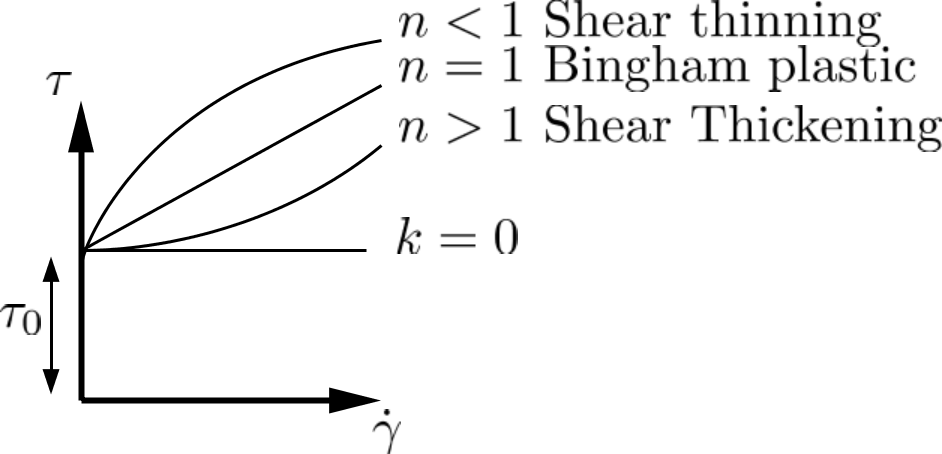
\includegraphics[width=.6\linewidth]{images/Non-newtonian.png}
	\end{center}
	\caption{Stress/strain-rate relationship for different flow index and consistency parameters in Herschel-Bulkley model.}
	\label{fig:HB}
\end{figure}
Subsequently, an apparent (effective) space-dependent viscosity satisfying $\tau = \mu_{eff}\dot{\gamma}$ and Eq.~\ref{eq:HB_t} may be defined \cite{WALLEVIK201495}
\begin{align}
\mu_{eff}= \tau_0/\dot{\gamma}+k \dot{\gamma}^{n-1}.
\label{eq:HB_mu}
\end{align}
Finally, the deviatoric stress in the momentum balance is written as $\bm{\sigma}^{dev} = 2 \mu_{eff} \bm E$, where $\bm E$ is defined in Eq.~\ref{eq:def_rate}. Given the incompressible flow assumption the, $\nabla  \bigcdot \bm \sigma^{dev}$ in Eqs.~\ref{eq:Cauchy_momentum_Eu}-\ref{eq:Cauchy_momentum_La} is written as follows:
\begin{align}
\nabla  \bigcdot \bm \sigma^{dev}&=\nabla \bigcdot (\mu_{eff} (\nabla\bf{u}+\nabla\bf{u}^T)) \nonumber\\
& = \mu_{eff} \nabla \bigcdot (\nabla \vect{u}) 
   +   \nabla \mu_{eff} \bigcdot \nabla \vect{u} 
+ \mu_{eff} \nabla (\nabla \bigcdot  \vect{u})
+ \nabla \mu_{eff}\bigcdot   \nabla  \vect{u}^T
\nonumber\\
& = \mu_{eff} \nabla^2 \vect{u}+   \nabla \mu_{eff} \bigcdot (\nabla \vect{u}+ \nabla  \vect{u}^T)
\label{eq:div_grad_u_NN}
\end{align}
The final form of the momentum balance for non-Newtonian fluids in Eulerian and Lagrangian frameworks respectively is as follows:
\begin{subequations}
	\begin{alignat}{2}
	\frac{\partial \rho \vect{u} }{\partial t}  + \vect{u} \bigcdot \nabla(\rho\vect{u}) + \nabla p- \mu\nabla^2 \vect{u}-
	 \nabla \mu_{eff} \bigcdot (\nabla \vect{u}+ \nabla  \vect{u}^T)
	-\vect{f}_b=0,\label{eq:NSE_Eulerian_NN}\\
	\frac{D (\rho \vect{u})}{D t}  + \nabla p- \mu\nabla^2 \vect{u}
	 -\nabla \mu_{eff} \bigcdot (\nabla \vect{u}+ \nabla  \vect{u}^T)
	  -\vect{f}_b=0,\label{eq:NSE_Lagrangian_NN}
	\end{alignat}
	\label{eq:NSE_NN}
\end{subequations}



\section{Discrete Systems}\label{sec:discrete_Model}
Contrary to continua, in discrete systems the motion of individual objects in the system and their interactions on each other is studied. In the following section the background information of such systems are described.
\subsection{Definitions}
For a reference on notation used in this and following sections please see Chapter \ref{chap:nomenclature}.
Throughout section \S\ref{sec:discrete_Model}, the following conventions are used to denote the quantities associated with discrete systems. Scalar variables are denoted by uppercase or lowercase lightface Latin and Greek letters, e.g. $\rho$ and $\phi$. Vectors are denoted via bold, lowercase Latin letters, e.g. $\vect{x}$ and they are column vectors unless otherwise specified. More specifically, the variables $\vect{x}$, $\vect{v}$, $\vect{a}$ are used to represent the position, velocity and acceleration of an object. Indexed vectors are used to specify either an element of the vector or an object in the vector depending on the context, e.g. $\vect{x}_i$ is the position of body $i$. The first time-derivative is represented with over dot, e.g. $\dot{\vect{x}} = \vect{v}$.  The second time-derivative is denoted via over double-dot, e.g. $\ddot{\vect{x}} = \dot{\vect{v}} = \vect{a}$.  Matrices are represented as bold uppercase Latin letters, e.g. $\matr{M}$. One subscript is used to specify a single row, e.g. $\matr{M}_i$ for row $i$ in the matrix $\matr{M}$. Two subscripts are used to indicate a specific row and column, e.g. $\matr{M}_{i,j}$.   
The Frobenius norm of a matrix or a vector is defined as $\|*\|_F$. The skew-symmetric cross product operator for a three dimensional vector is defined as follows and results in a $3\times 3$ matrix
\begin{equation}
\tilde{{\vect s}} = \begin{bmatrix}
0 & -{s}_z & {s}_y\\ 
{s}_z & 0 & -{s}_x\\ 
-{s}_y & {s}_x & 0.
\end{bmatrix}
\end{equation}
\subsection{Rigid Body Dynamics}\label{sec:RigidBody}
In this section we describe the dynamic systems featuring rigid bodies and frictional contact between them. As explained in Section \S\ref{sec:back_rigid}, a complementarity-based approach is used to resolve the contact between different objects. 

\subsubsection*{Preamble}
``Rigid body" refers to a 3D object that can translate and rotate in space. The set of generalized coordinates that describe the position and orientation of a body in the 3D Euclidean space are $\br_j\in \mathbb{R}^3$ and $\vect{\epsilon}_j\in \mathbb{R}^4$, which are respectively the absolute position of the center of mass, and Euler parameters associated with orientation of body $j$. Combining the set of generalized coordinates of different bodies for a system of $n_b$ bodies, one can write the set of generalized coordinates describing the system at position level as $\vect{x} = \left[ \vect{r}_1^T, \vect{\epsilon}_1^T,\ldots,\vect{r}_{n_b}^T, \vect{\epsilon}_{n_b}^T \right]^T \in \mathbb{R}^{7 n_b} $, and at velocity level as  $\dot{\vect{x}} = \left[ \dot{\vect{r}}_1^T, \dot{\vect{\epsilon}}_1^T,\ldots, \dot{\vect{r}}_{n_b}^T, 
\dot{\vect{\epsilon}}_{n_b}^T \right]^T$ $\in \mathbb{R}^{7 n_b}$. One can choose to use angular velocities instead of the time derivative of the Euler parameters to describe the system at the velocity level by  $\vect{v} = \left[ \dot{\vect{r}}_1^T, \bar{\vect{\omega}}_1^T,\ldots, \dot{\vect{r}}_{n_b}^T, 
\bar{\vect{\omega}}_{n_b}^T \right]^T$ $\in \mathbb{R}^{6 n_b}$, which reduces the problem size. The transformation from the derivatives of Euler parameters, ${\dot{\vect{\epsilon}}}_{B}$, to angular velocities at the body-fixed frame, ${\bar{\vect{\omega}}}_{B}$, for each body is governed by ${\dot{\vect{\epsilon}}}_{B}=\frac{1}{2} {\matr{G}}^T(\vect{\epsilon}_{B}) {\bar{\vect{\omega}}}_{B} $, where matrix ${\matr{G}}\in {\mathbb{R}}^{3 \times 4}$ depends linearly on the Euler parameters ${\vect{\epsilon}}_{B}$. Therefore, if one chooses to work with Euler angles at the velocity level, the block diagonal matrix  ${\vect L}(\vect{q}) \equiv \mbox{diag} \left[{{\matr I}}_{3 \times 3}, \frac{1}{2} {\matr{G}}^T(\vect{\epsilon}_{1}),\ldots,{\matr I}_{3 \times 3}, \frac{1}{2} {\matr{G}}^T(\vect{\epsilon}_{n_b})\right] \in {\mathbb{R}}^{7 n_b \times 6 n_b}$ can be used to obtain ${\dot{\vect{x}}} = {\vect L}({\vect{q}}) \vect{v}$, the time derivative of the set of generalized coordinate describing the system, where ${\matr I}_{3 \times 3}$ is the identity matrix \cite{Haug89}. 

\subsubsection*{The DVI Formulation of the Frictional Contact Problem}
In Differential Variational Inequality (DVI) \cite{pastew03dvi} approach the equations of motion are modified to include the differential inclusion \cite{filippov1967classical} and to impose non-penetration between rigid bodies through constraints enforced by applying impulses. After discretization this problem is posed as an optimization problem with complementarity and equilibrium constraints. More specifically, the three-dimensional Coulomb friction assumption leads to a Non-linear Complementarity Problem (NCP).  In what follows, more details about the theory of the complementarity approach is explained.

Consider a contact between bodies $A$ and $B$ as shown in Fig.~\ref{fig:DVI_Contact}. The tangent plane at the contact point for the contact $i$ is defined by vectors $\textbf{u}_i$, $\textbf{w}_i$ and the normal $\textbf{n}_i$ in Fig.~\ref{fig:DVI_Contact}. A local reference frame can be defined for each body at the contact point based on these vectors. For body $A$, the normal to the tangent plane, $\textbf{n}_{i,A}$, points toward body $B$. The two mutually orthogonal vectors $\textbf{u}_{i,A}$, and $\textbf{w}_{i,A}$ are defined using the Gram-Schmidt method. The same methodology is used to build the local reference frame at the contact point $i$, for body $B$ with $\textbf{w}_{i,B}$, $\textbf{u}_{i,B}$, and $\textbf{n}_{i,B}$ $\in \mathbb{R}^3$. 

\begin{figure}
	\begin{center}
		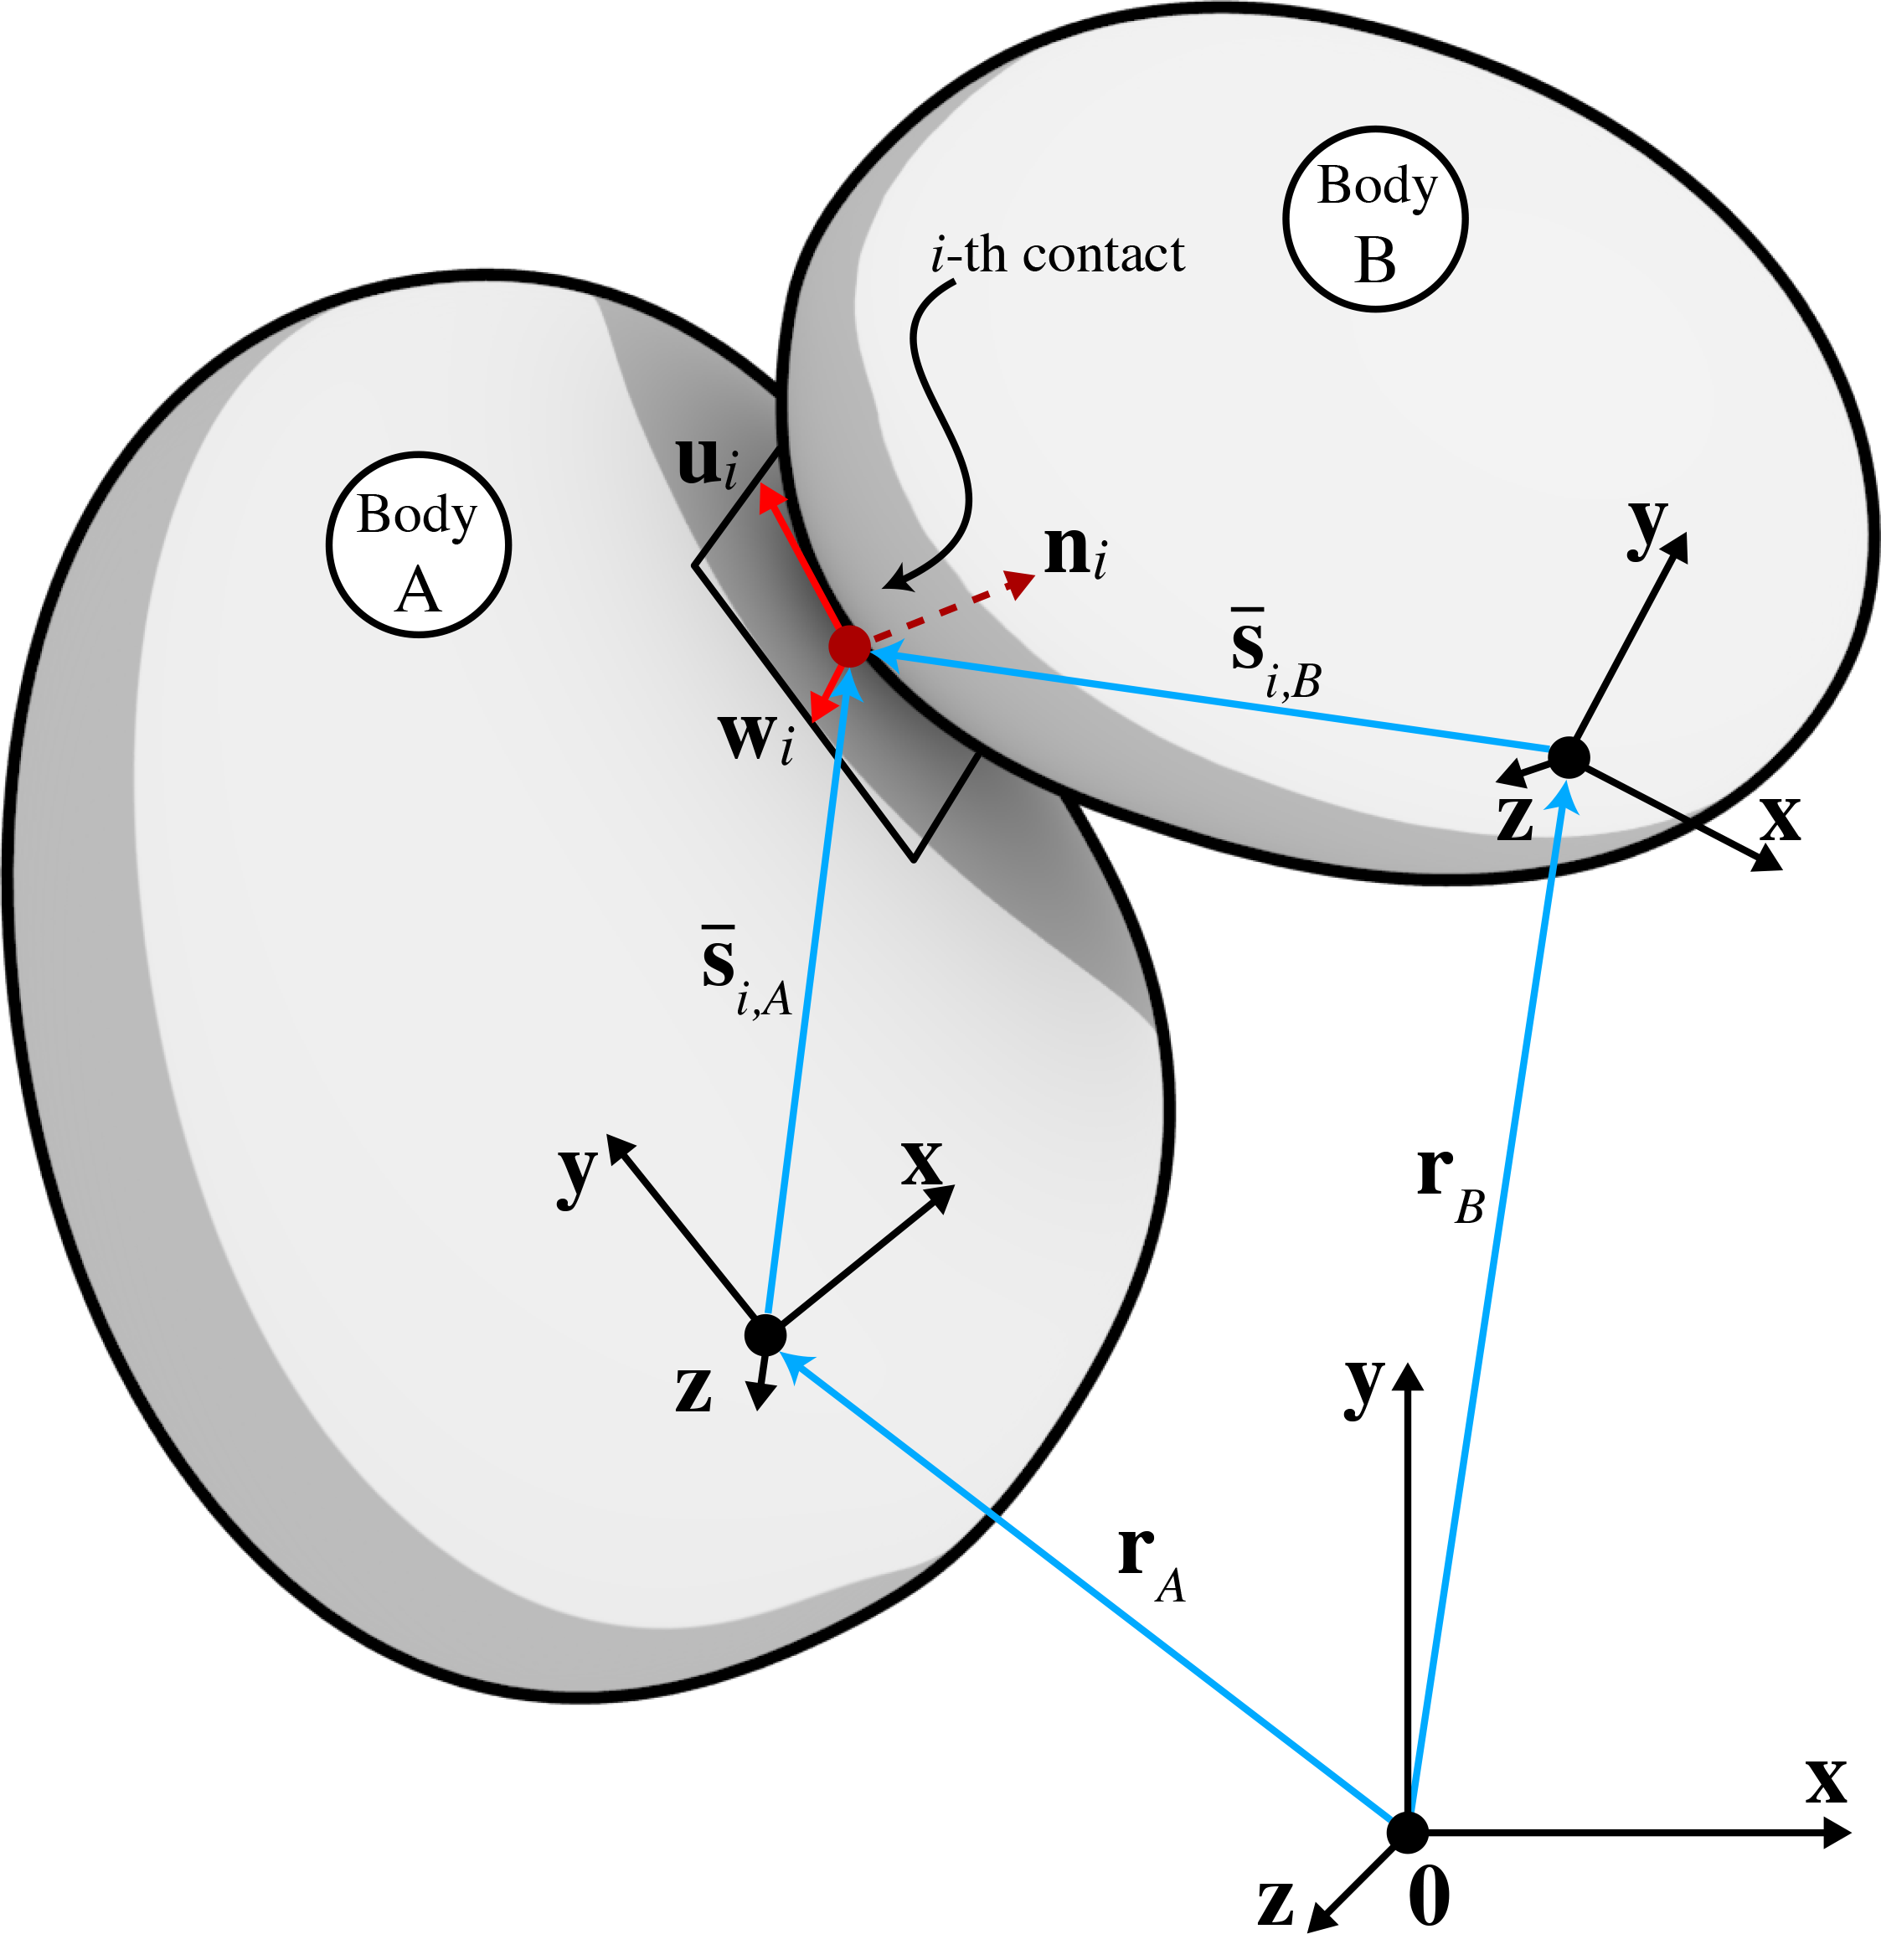
\includegraphics[width=.4\linewidth]{images/twobodies.png}
	\end{center}
	\caption{Schematic of contact between two bodies.}
	\label{fig:DVI_Contact}
\end{figure}

If the gap (distance) between bodies $A$ and $B$ at the contact point is defined by $\Phi$, a complementarity condition can be defined as $0 \leq \widehat{\gamma}^c_{i,n}  \perp \Phi \geq 0$, where $\widehat{\gamma}^c_{i,n}$  is the Lagrange multiplier associated with the contact $i$. The complementarity condition states that at least one of the $\widehat{\gamma}^c_{i,n}$, or $\Phi$ is zero; when the gap function is zero, the normal contact force is greater than zero and when the normal contact force is zero the gap function is greater than zero (there is no contact between body $A$ and $B$). The contact force associated with contact $i$ can be expressed as $\vect{f}_{i,N}=\widehat{\gamma}^c_{i,n}\vect{n}_i$, and $\vect{f}_{i,T}=\widehat{\gamma}^c_{i,u}\vect{u}_i+\widehat{\gamma}^c_{i,w}\vect{w}_i$ which are the normal and tangential forces, respectively.  $\widehat{\gamma}^c_{i,w}$, $\widehat{\gamma}^c_{i,u}$, and $\widehat{\gamma}^c_{i,n}$ are the magnitude of the contact forces in each direction. The Coulomb dry-friction model based on the friction forces is expressed as  \cite{StTr95,stewartSIAMreview2000}
\begin{subequations}
	\begin{align}
	\label{eq:FrictionModel_1}
	\sqrt{(\widehat{\gamma}^c_{i,u})^2+(\widehat{\gamma}^c_{i,w})^2}\leq \mu^f_{i} \widehat{\gamma}^c_{i,n}&,\\ 
	\label{eq:FrictionModel_2}
	\quad \lVert\vect{v}_{i,T}\rVert\left(\sqrt{(\widehat{\gamma}^c_{i,u})^2+(\widehat{\gamma}^c_{i,w})^2} - \mu^f_{i} \widehat{\gamma}^c_{i,n} \right)=0&,\\
	\label{eq:FrictionModel_3}
	\langle\vect{f}_{i,T},\vect{v}_{i,T}\rangle=-\lVert\vect{f}_{i,T}\rVert\lVert\vect{v}_{i,T}\rVert \;&,
	\end{align}
\end{subequations}
where $\vect{v}_{i,T}$ denotes the relative tangential velocity between bodies $A$ and $B$ at the contact point. More specifically, Eq.~\ref{eq:FrictionModel_1} states that the the friction force is less than the normal force times the friction coefficient.  Eq.~\ref{eq:FrictionModel_2} states a complementarity condition where equality condition of Eq.~\ref{eq:FrictionModel_1} holds if the $\vect{v}_{i,T}\not=0$, and inequality of Eq.~\ref{eq:FrictionModel_1} holds if $\vect{v}_{i,T}=0$. Lastly, Eq.~\ref{eq:FrictionModel_3} states that the friction force is in the opposite direction of $\vect{v}_{i,T}$. If now one considers the following constraint minimization problem, 
\begin{equation}
\label{eq:fricMin}
\left( \widehat{\gamma}^c_{i,u},\widehat{\gamma}^c_{i,w} \right) = \mathop {\mbox{argmin}}\limits_{\sqrt{(\widehat{\gamma}^c_{i,u})^2+(\widehat{\gamma}^c_{i,w})^2} \leq \mu^f_{i} \widehat{\gamma}^c_{i,n}}
{\mathbf v}_{i,T}^T \left( \widehat{\gamma}^c_{i,u} \uVec{i} + \widehat{\gamma}^c_{i,w} \wVec{i} \right),
\end{equation}
then Eq.~\ref{eq:FrictionModel_1}-\ref{eq:FrictionModel_3} represent the first order Karush-Kuhn-Tucker optimality condition for the above optimization problem with respect to $\widehat{\gamma}^c_{i,u}$, and $\widehat{\gamma}^c_{i,w}$ variables. Hence, the Coulomb friction model is implemented as a constraint optimization problem. Finally, the contact force at the $i^{th}$ contact point is expressed as $\vect{f}_i=\vect{f}_{i,N}+\vect{f}_{i,T}=\widehat{\gamma}^c_{i,n}\vect{n}_i+\widehat{\gamma}^c_{i,w}\vect{u}_i+\widehat{\gamma}^c_{i,w}\vect{w}_i \in \cone_i$,  where $\cone_i$ is a 3D cone of slope $\tan^{-1}(\mu^f_{i})$ and oriented along $\vect{n}_i$, i.e., $\cone_i=\{\left[x,y,z\right]^T \in \mathbb{R}^3 | \sqrt{y^2+z^2} \leq \mu^f_{i} x\}$.


The Newton-Euler equations of motion for the system \cite{StTr95} are expressed as:
\begin{equation}
\label{eq:Newton_Euler}
\begin{gathered}
\begin{array}{rcl}
{\mathbf{\dot q}}   & = &  {\bf L}({\mathbf{q}}){\bf v} \vspace{0.2cm}  \\ 
{\mathbf{M}} {\mathbf{\dot v}} & = &{\mathbf{f}}\left( {t,  {\bf q} , {\bf v} } \right) -\vect{g}_{\vect{q}}^T\left(\vect{q},t\right)\lambda  + \vspace{0.2cm} \sum\limits_{i\in \cA({\bf q},\delta)} \left( \hatGN{i} \Pn{i} + \hatGU{i} \Ptu{i}  + \hatGW{i} \Ptw{i}  \right) \vspace{0.2cm} \\
0 & = & {\bf g}({\bf q},t)\vspace{0.2cm}  \\ 
i \in \cA({\bf q}(t),\delta)  &:&  0 \le \hatGN{i} \; \perp \; \Phi_{i}({\bf q}) \geq 0 \vspace{0.2cm} \\
\left(\hatGU{i}, \hatGW{i} \right)  &=&  \mathop {\mbox{argmin}}\limits_{\sqrt{(\widehat{\gamma}^c_{i,u})^2+(\widehat{\gamma}^c_{i,w})^2} \leq \mu^f_{i} \widehat{\gamma}^c_{i,n}} {\bf v}^T \left( \widehat{\gamma}^c_{i,u} \Ptu{i} + \widehat{\gamma}^c_{i,w} \Ptw{i} \right) \;,
\end{array}
\end{gathered} 
\end{equation}
where  $\mathbf{f}(t,  {\bf q} , {\bf v} ) $ are the external forces, $\textbf{M}$ is the system mass Matrix, $\cA({\bf q},\delta)$  is the set of active and potential unilateral constraints based on the bodies that are mutually less than $\delta$ apart, and $\textbf{g}(\textbf{q},t)$ is the set of bilateral constraints acting on the system and $\vect{g}_{\vect{q}}^T\left(\vect{q},t\right)$ is the Jacobian of the constraints with respect to the generalized coordinates. Moreover, the tangent space generators 
$\Proj{i}=[\Pn{i}, \Ptu{i}, \Ptw{i} ] \in {\mathbbm{R}}^{6n_b \times 3}$ are defined as
%
\begin{equation}
\begin{gathered}
\Proj{i}^{T} =
\left[ 
{\bf 0} \;\; \ldots \;\; - {\bf A}_{i,p}^T \;\; { {\bf A}_{i,p}^T {\bf{A}}_A {\tilde {\bar {\bf{s}}}}_{i,A}}  
\;\; {\bf 0} \;\;  \ldots  \;\;  {\bf 0} \;\;
{\bf A}_{i,p}^T \;\; { - {\bf A}_{i,p}^T {\bf{A}}_B  {\tilde {\bar {\bf{s}}}}_{i,B}  }  \;\; \ldots \;\;{\bf 0}
\right] ,
\end{gathered} 
\end{equation}
%
where ${\bf{A}}_{i,p} = [\nVec{i}, \uVec{i}, \wVec{i} ] \in {\mathbbm{R}}^{3 \times 3}$ is the orientation matrix associated with contact $i$,
${\bf{A}}_A={\bf{A}}\left({\bf \epsilon}_A\right)$ and ${\bf{A}}_B={\bf{A}}\left({\bf \epsilon}_B\right)$ are the rotation matrices of bodies $A$ and $B$ respectively; the vectors ${\bar {\bf s}}_{i,A}$ and ${\bar {\bf s}}_{i,B} \in {\mathbbm{R}}^{3}$  represent the contact point positions in body-relative coordinates as shown in Fig.~\ref{fig:DVI_Contact}. More details about the solution algorithm, and time-stepping scheme of the this DVI problem may be found in \cite{StTr95,ani04,aniha03}.


\subsection{Flexible Body Dynamics}
The nonlinear flexible body dynamics formulation used in the current work draws on ANCF, a nonlinear finite element formulation introduced by Shabana~\cite{Shabana1997} to describe large deformation of moving bodies. The salient feature of ANCF is the use of position vector gradients to describe the rotation of the body. ANCF uses nodal global position and nodal position vector gradient vectors to describe the nonlinear dynamics of flexible bodies that can undergo large deformation.
In general, the position field of $i^{th}$ ANCF element may be defined as: 
\begin{equation} \label{eq:ANCF_r}
\underbrace{{{\bm{r}}^{i}}(\xi,\eta,\zeta,t)}_{\begin{smallmatrix}
	\text{Position of an arbitrary } \\
	\text{point within the element}
	\end{smallmatrix}}=\underbrace{\bm{S}(\xi,\eta,\zeta)}_{\begin{smallmatrix}
	\text{Space-dependent } \\
	\text{shape function}
	\end{smallmatrix}}\times \underbrace{{{\bm{q}}^{i}}(t),}_{\begin{smallmatrix}
	\text{Time-dependent vector of } \\
	\text{nodal degrees of freedom}
	\end{smallmatrix}}
\end{equation}
which simply gives the position of any point $(\xi,\eta,\zeta) \in [-1,1]$ inside the element at time $t$ based on interpolation ($\bm{S} (\xi,\eta,\zeta) $) of the nodal coordinates ($\bm{q}^{i}(t)$). Due to the fact that description of elements is in global coordinates, the inertia forces have a simple form in ANCF elements. The velocity of any point within an element $i$ may be written as
\begin{equation} \label{eq:ANCF_r_dot}
\underbrace{\bm{\dot{r}}^{i}(\xi,\eta,\zeta,t)}_{\begin{smallmatrix}
	\text{Velocity of an arbitrary } \\
	\text{point within the element}
	\end{smallmatrix}}=\underbrace{\bm{S}(\xi,\eta,\zeta)}_{\begin{smallmatrix}
	\text{Space-dependent } \\
	\text{shape function}
	\end{smallmatrix}}\times \underbrace{\bm{\dot{q}}^{i}(t).}_{\begin{smallmatrix}
	\text{Time-dependent vector of } \\
	\text{generalized velocities}
	\end{smallmatrix}}
\end{equation}
The kinetic energy of a finite element $i$ can be obtained as
\begin{equation} \label{eq:ANCF_T}
T = \frac{1}{2}\int\limits_V {\rho {{{\mathbf{\dot r}}}^{i\text{T}}}{\mathbf{\dot r}}^{i}} {\text{ d}}V = \frac{1}{2}{{\mathbf{\dot q}}^{i\text{T}}}{\mathbf{M\dot q}^{i}}\;,
\end{equation}
where the mass matrix ${\mathbf{M}}$ is defined as \small ${\mathbf{M}} = \int_A {\rho A {{\bm{S}}^\text{T}}{\bm{S}}} {\text{ d}}x$, which is time-independent. The equations of motion assume the form \cite{shabana2013} 
\begin{equation}
\mathbf{M} \ddot{\mathbf{q}} + \mathbf{{Q}}_e=\mathbf{{Q}}_a\;,
\end{equation}
where  $\mathbf{{Q}}_e$ and $\mathbf{{Q}}_a$ are the generalized element elastic and applied forces, respectively. The description of these elements and calculation of the internal forces are described in \S \ref{sec:1DElem}, and \S \ref{sec:2DElem}.

ANCF elements may be classified based on the number of position vector gradients defined at each node. ($i$) \textbf{Fully parameterized} ANCF elements use position vector $r \in \mathbb R^3$, and 3 position vector gradients, $\bm{r}_x$, $\bm{r}_y$, and $ \bm{r}_z  \in \mathbb R^3 $ where $x$, $y$, and $z$ are the natural coordinates of the element. Fully parameterized elements allow for easy implementation of the continuum mechanics approach to calculate the deformation gradient ($\textbf{F}$). ($ii$) \textbf{Gradient Deficient} ANCF elements use position vector $r \in \mathbb R^3$, and fewer than 3 position vector gradients, when using fewer position vector gradients is sufficient to define the volume used in continuum mechanics approach. Using fewer position gradient vectors has been shown to eliminate various locking problems.

Development of ANCF elements is still an ongoing research topic, yet in the current work elements that have been shown robust and acceptable accuracy  are chosen for the simulations of the flexible bodies. More specifically, ANCF cable element, ANCF shell element, and hexahedron brick elements, which are appropriate respectively for modeling 1D, 2D, and 3D bodies, are to be used in the FE analysis of this present work.


\subsubsection*{ANCF Cable Element}\label{sec:1DElem}
The gradient-deficient ANCF cable element introduced by Berzeri and Shabana~\cite{berzeri2000} is used in the present work. As shown in Fig.~\ref{fig:ANCFCable}, the coordinates of this element at each node are a position vector and a position vector gradient along the beam center axis. The position gradient vectors normal to the cable axis are not defined, hence the element is gradient deficient. Subsequently, torsion and shear deformation cannot be captured with this set of degrees of freedom. The coordinates (nodal degree of freedom) of the $j^{th}$ node is expressed as the $6 \times 1$ matrix \small${{\bm{q}}^{j}}(t)={{\left[ \begin{matrix}
		\bm{r}_{{}}^{j\text{T}} & \bm{r}_{x}^{j\text{T}}  \\
		\end{matrix} \right]}^{\text{T}}}$. \normalsize The position of any point inside the $i^{th}$ element may be interpolated from the nodal degrees of freedom of its nodes as follows
\begin{equation} \label{eq:ANCF_Beam_r}
\bm{r}^{i}=\left[ \begin{matrix}
{{s}_{1}}\bm{I} & {{s}_{2}}\bm{I} & {{s}_{3}}\bm{I} & {{s}_{4}}\bm{I}  \\
\end{matrix} \right]\left[ \begin{matrix}
\bm{q}_{}^{1\text{T}} & \bm{q}_{}^{2\text{T}}  \\
\end{matrix} \right]^\text{T}=\bm{S}\left( \xi  \right)\bm{q}^{i},
\end{equation}
where $\bI$ is the $3\times3$ identity matrix, $\bm{S}\left( \xi  \right)$ is a $3 \times 12$ matrix, $\bm{q}^1$, are $\bm{q}^2$ are the nodal coordinates of the two nodes forming element $i$, as defined before, and finally $\bm{q}^{i}$ is a $12\times1$ matrix combining the nodal coordinates of the element $i$. The interpolation functions are defined as
\begin{equation} \label{eq:ANCF_Beam_Shapefunctions}
\begin{split}
& {{s}_{1}}=1-2{{\xi}^{2}}+2{{\xi}^{3}}, \\
& {{s}_{2}}=l\left( \xi-2{{\xi}^{2}}+{{\xi}^{3}} \right), \\
& {{s}_{3}}=3{{\xi}^{2}}-2{{\xi}^{3}}, \\
& {{s}_{4}}=l\left( -{{\xi}^{2}}+{{\xi}^{3}} \right), \\
\end{split}
\end{equation}
where $0<\xi <1$ is the non-dimensional parameter defined over the natural coordinates of the element locates a point along the cable centerline ($\xi=0$ at the first node, and $\xi=l$ at the second node), and $l$ is the length of the element.

\begin{figure}[!t]
	\begin{center}
				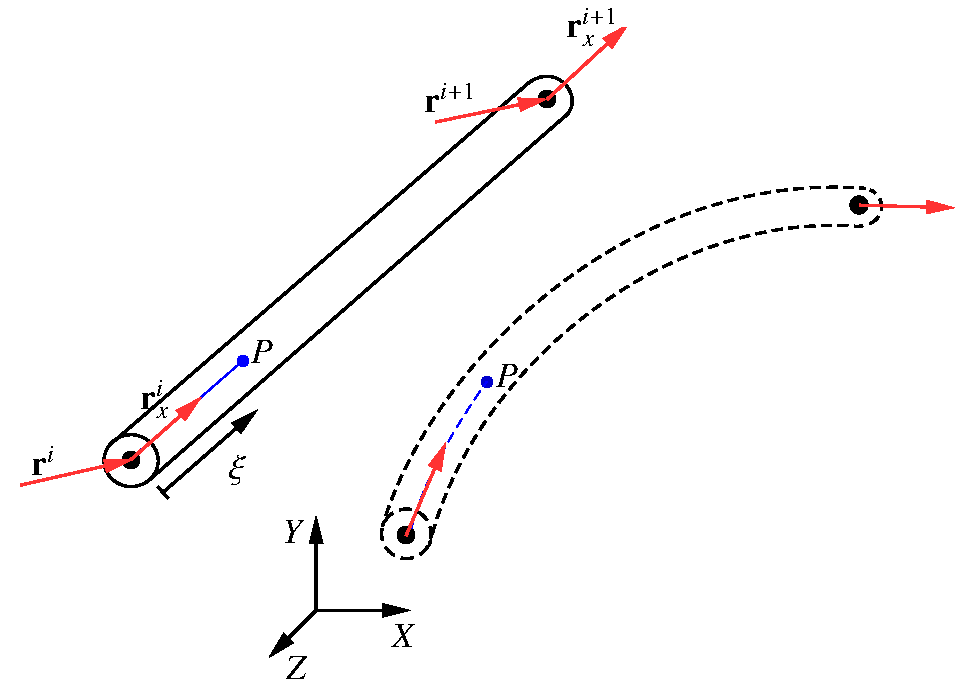
\includegraphics[width=.6\linewidth]{images/ANCF_1D.pdf}
	\end{center}
\caption{ANCF cable element's schematic. Each node features a global position vector and a position vector gradient along the axis of the element (6DOF). Using shape functions and knowing $\xi$ one can interpolate the degrees of freedom to any point $P$ within the element. } \label{fig:ANCFCable}
\end{figure}


Knowing the axial and bending strains, one can define the internal loads of this element. 
The generalized element elastic forces are calculated as follows:
\begin{equation} \label{eq:ANCF_Beam_Qe}
\mathbf{Q}^i_{e}=\int\limits_{L}{\left[ EA \varepsilon_{x} ({\frac{{\partial \varepsilon }_{x}}{\partial \mathbf{q}}})^T+EI\kappa ({\frac{\partial \kappa}{\partial \mathbf{q}}})^T  \right]}\text{d}x,
\end{equation}
where $E$, $A$, and $I$ are the modulus of elasticity, the cross section area, and the area moment of inertia, respectively. The axial strain and curvature are defined as follows
\begin{equation*} \label{eq:ANCF_Beam_ex_k}
{{\varepsilon }_{x}}=\frac{1}{2}\left( \bm{r}_{x}^{\text{T}}\bm{r}_{x}^{{}}-1 \right) \text{  } \text{and} \text{  } \kappa \text{=}\frac{\left| {{\bm{r}}_{x}}\times {{\bm{r}}_{xx}} \right|}{{{\left| {{\bm{r}}_{x}} \right|}^{3}}},
\end{equation*}
where $\bm{r}^i_{x}=\bm{S}_x(\zeta) \bm{q}^i$ and $\bm{r}^i_{xx}=\bm{S}_{xx}(\zeta) \bm{q}^i$ terms involve differentiation of the shape function matrix $\bm S$.

Similarly, external applied forces, including those coming from the fluid system are interpolated to nodal coordinates and subsequently applied in the structural system via:
 \begin{equation} \label{eq:ANCF_Beam_Qa}
 Q^i_a = \bm S(x)^T \bm F.
 \end{equation}

The generalized body forces including gravity force may be computed according to the standard finite element formulation as :

 \begin{equation} \label{eq:ANCF_Beam_Qb}
Q^i_b = \int_{L} \rho_s A \bm S(x)^T \bm f_b,
\end{equation}
where $\rho_s$ and $A$ are the density and cross sectional area of the element, and $f_b$ is density of the body force. 


\subsubsection*{ANCF Shell Element}\label{sec:2DElem}
The gradient-deficient ANCF shell element studied in \cite{Yamashita2015continuum} is used in the present work to simulate 2D flexible bodies. The nodal global position vector ($\mathbf{r}^{i}$) and global position vector transverse gradient ($\mathbf{r}_{z}^{i}=\frac{\partial {{\mathbf{r}}^{i}}}{\partial {{z}^{i}}}({{\xi}^{i}},{{\eta}^{i}})$) are chosen as the nodal degrees of freedom, as shown in Fig.~\ref{fig:ANCF_Shells}.

\begin{figure}[!t]
	\begin{center}
				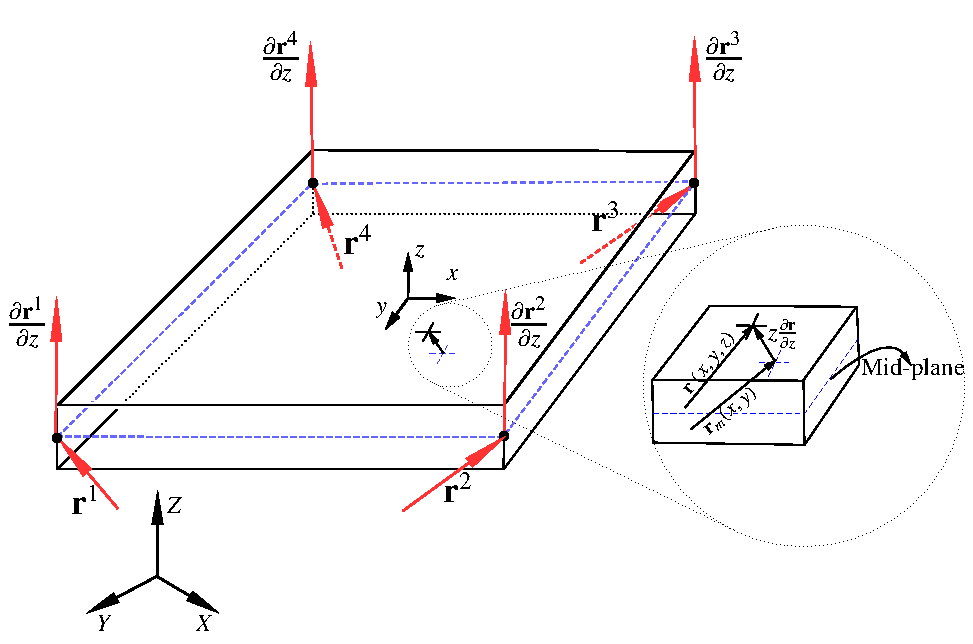
\includegraphics[width=.6\linewidth]{images/ANCF_2D.pdf}
	\end{center}
		\caption{ANCF shell element's schematic. Global position vector $\mathbf{r}^{j}$ and fiber's direction $\mathbf{r}_z^{j}=\frac{\partial {{\mathbf{r}}^{j}}}{\partial {{z}^{i}}}({{\xi}^{i}},{{\eta}^{j}})$ are the nodal coordinates of the $j^{th}$ node (6DOF). Using shape functions and knowing $\xi$ and $\eta$ one can interpolate the degrees of freedom to any point within the element. }\label{fig:ANCF_Shells}
\end{figure}

The positions and gradients on the mid-plane for any point inside the $i^{th}$ element can be interpolated from the positions and gradients of its nodes as follows
\begin{equation} \label{eq:ANCF_Shell_coordinates}
\mathbf{r}_{m}^{i}({{\xi}^{i}},{{\eta}^{i}})=\mathbf{S}_{m}^{i}({{\xi}^{i}},{{\eta}^{i}})\mathbf{e}_{p}^{i},\quad \frac{\partial {{\mathbf{r}}^{i}}}{\partial {{z}^{i}}}({{\xi}^{i}},{{\eta}^{i}})=\mathbf{S}_{m}^{i}({{\xi}^{i}},{{\eta}^{i}})\mathbf{e}_{g}^{i},
\end{equation}
where $\xi^i$ and $\eta^i$ refer to $i^{th}$ element's natural coordinates in the parametric space, $\mathbf{S}_{m}^{i}=\begin{bmatrix}
S_{1}^{i}\mathbf{I}& S_{2}^{i}\mathbf{I}& S_{3}^{i}\mathbf{I}&  S_{4}^{i}\mathbf{I}] \end{bmatrix}$ is a bilinear shape function matrix, $\mathbf{e}_{p}^{ij}={{\mathbf{r}}^{ij}}$ is the position vector of $j^{th}$ node of the element $i$, and $\mathbf{e}_{g}^{ij}={\partial {{\mathbf{r}}^{ij}}}/{\partial {{z}^{i}}}\;$ is the position vector gradient of node $j$ of element $i$, and $\textbf{I}$ is the $3\times 3$ identity matrix.
The bilinear shape functions of the ANCF shell element are given by the following expressions
\begin{equation*} \label{eq:ANCF_Shell_Shapefunctions}
\begin{split}
S_{1}^{i}=\frac{1}{4}(1-{{\xi }^{i}})(1-{{\eta }^{i}}), S_{2}^{i}=\frac{1}{4}(1+{{\xi }^{i}})(1-{{\eta }^{i}}),\\
S_{3}^{i}=\frac{1}{4}(1+{{\xi }^{i}})(1+{{\eta }^{i}}), S_{4}^{i}=\frac{1}{4}(1-{{\xi }^{i}})(1+{{\eta }^{i}}).
\end{split}
\end{equation*}
The position of an arbitrary point in the $i^{th}$ element may be described as
\begin{equation} \label{eq:ANCF_Shell_r}
{{\mathbf{r}}^{i}}({\xi}^i,{\eta}^i,{z}^i)={{\mathbf{S}}^{i}}({\xi}^i,{\eta}^i,{z}^i){{\mathbf{e}}^{i}},
\end{equation}
where ${{\mathbf{S}}^{i}}=[\begin{matrix} \mathbf{S}_{m}^{i} \,\,\, {{z}^{i}}\mathbf{S}_{m}^{i}\end{matrix}]_{3\times 24}$ is the combined shape function matrix, and $\quad {{\mathbf{e}}^{i}}= [{ \begin{matrix} {{(\mathbf{e}_{p}^{i})}^{T}} \,\,\, {{(\mathbf{e}_{g}^{i})}^{T}}\end{matrix}}]_{1\times 24}^T$ is the coordinates of the $i^{th}$ element grouped together. Eq.~\ref{eq:ANCF_Shell_r} allows for interpolating points along the element thickness by incorporating the element natural coordinate $z^i$.
The Green-Lagrange strain tensor, which is expressed as follows, 
\begin{equation} 
{{\mathbf{E}}^{i}}=\frac{1}{2}\left( {{\left( {{\mathbf{F}}^{i}} \right)}^{T}}{{\mathbf{F}}^{i}}-\mathbf{I} \right),
\label{eq:ANCF_E}
\end{equation}
is used to obtain the strains, where ${\mathbf{F}}^{i}$ is the deformation gradient matrix defined as the Jacobian of the current configuration over the reference configuration, which is expressed as 
\begin{equation} 
{{\mathbf{F}}^{i}}=\frac{\partial {{\mathbf{r}}^{i}}}{\partial {{\mathbf{X}}^{i}}}=\frac{\partial {{\mathbf{r}}^{i}}}{\partial {{\mathbf{x}}^{i}}}{{\left( \frac{\partial {{\mathbf{X}}^{i}}}{\partial {{\mathbf{x}}^{i}}} \right)}^{-1}}=  \bar {\bm J}^i  ({\bm J^i})^{-1}, \label{eq:ANCF_F}
\end{equation}
where $\dfrac{\partial {{\mathbf{r}}^{i}}}{\partial {{\mathbf{x}}^{i}}}=\bar {\bm J}^i$, and ${{ \dfrac{\partial {{\mathbf{X}}^{i}}}{\partial {{\mathbf{x}}^{i}}} }}= {\bm J^i}$. Incorporating \ref{eq:ANCF_F}, in \ref{eq:ANCF_E} results in
\begin{equation}
\bm{E}^i=({\bm{J}^i})^{-T} \tilde{\bm{E}}^i ({\bm{J}^i})^{-1},
\label{eq:ANCF_E2}
\end{equation}
where $\tilde{\bm{E}}^i$ the covariant strain tensor defined via:
\begin{equation}
{\tilde{\bm{E}}}^i=\frac{1}{2}\big( (\bar {\bm J}^i)^{T}  \bar {\bm J}^i -  (\bm J^i)^{T}  {\bm J}^i  \big)
\label{eq:ANCF_E_tilde}
\end{equation}
and can be re-expressed in a vector form as follows:
\begin{equation} \label{eq:equ7}
{{\bm{\tilde{\varepsilon} }}^{i}}={{\left[ \begin{matrix}
		\tilde{\varepsilon} _{xx}^{i} & \tilde{\varepsilon} _{yy}^{i} & \tilde{\gamma} _{xy}^{i} & \tilde{\varepsilon} _{zz}^{i} & \tilde{\gamma} _{xz}^{i} & \tilde{\gamma} _{yz}^{i} \\
		\end{matrix} \right]}^{T}}
\end{equation}
The engineering strain vector can be expressed in terms of the covariant strain vector as follows:
\begin{equation}
{{\bm{\varepsilon }}^{i}}=(\bm {T}^i)^{-T} {{\bm{\tilde{\varepsilon} }}^{i}}
\end{equation}
where the  engineering strain vector in the deformed configuration is defined via  
\begin{equation} \label{eq:equ8}
{{\bm{\varepsilon }}^{i}}={{\left[ \begin{matrix}
		\varepsilon _{xx}^{i} & \varepsilon _{yy}^{i} & \gamma _{xy}^{i} & \varepsilon _{zz}^{i} & \gamma _{xz}^{i} & \gamma _{yz}^{i} \\
		\end{matrix} \right]}^{T}}.
\end{equation}
 Above, the constant transformation matrix (note that ${{\mathbf{J}}^{i}}$ only depends on the initial and reference configuration).
\begin{equation} \label{eq:equ10}\scriptsize
{{\mathbf{T}}^{i}}=\left[ \begin{matrix}
{{(J_{11}^{i})}^{2}} & {{(J_{12}^{i})}^{2}} & 2J_{11}^{i}J_{12}^{i} & {{(J_{13}^{i})}^{2}} & 2J_{11}^{i}J_{13}^{i} & 2J_{12}^{i}J_{13}^{i}  \\
{{(J_{21}^{i})}^{2}} & {{(J_{22}^{i})}^{2}} & 2J_{21}^{i}J_{22}^{i} & {{(J_{23}^{i})}^{2}} & 2J_{21}^{i}J_{23}^{i} & 2J_{22}^{i}J_{23}^{i}  \\
J_{11}^{i}J_{21}^{i} & J_{12}^{i}J_{22}^{i} & J_{11}^{i}J_{22}^{i}+J_{12}^{i}J_{21}^{i} & J_{13}^{i}J_{23}^{i} & J_{11}^{i}J_{23}^{i}+J_{13}^{i}J_{21}^{i} & J_{12}^{i}J_{23}^{i}+J_{13}^{i}J_{22}^{i}  \\
{{(J_{31}^{i})}^{2}} & {{(J_{32}^{i})}^{2}} & 2J_{31}^{i}J_{32}^{i} & {{(J_{33}^{i})}^{2}} & 2J_{31}^{i}J_{33}^{i} & 2J_{32}^{i}J_{33}^{i}  \\
J_{11}^{i}J_{31}^{i} & J_{12}^{i}J_{32}^{i} & J_{11}^{i}J_{32}^{i}+J_{12}^{i}J_{31}^{i} & J_{13}^{i}J_{33}^{i} & J_{11}^{i}J_{33}^{i}+J_{13}^{i}J_{31}^{i} & J_{12}^{i}J_{33}^{i}+J_{13}^{i}J_{32}^{i}  \\
J_{21}^{i}J_{31}^{i} & J_{22}^{i}J_{32}^{i} & J_{21}^{i}J_{32}^{i}+J_{22}^{i}J_{31}^{i} & J_{23}^{i}J_{33}^{i} & J_{21}^{i}J_{33}^{i}+J_{23}^{i}J_{31}^{i} & J_{22}^{i}J_{33}^{i}+J_{23}^{i}J_{32}^{i}  \\
\end{matrix} \right]\normalsize
\end{equation}
The elastic internal forces are obtained by integration over the element volume using Gaussian quadrature as follows
\begin{equation} \label{eq:equ11}
\mathbf{Q}_{e}^{i}=\int\limits_{V_0^i}{\left( \frac{\partial {{\mathbf{\varepsilon }}^{i}}}{\partial {{\mathbf{e}}^{i}}} \right)^T} \sigma ^i \text{d}{{V}_{0}^i}\;,
\end{equation}
where $\mathbf{\sigma}^{i}$ is the vector of the second Piola-Kirchhoff stresses and $dV_i^0$ is the infinitesimal volume at the reference configuration of the element $i$.  

In order to alleviate the locking of the element, two modifications are performed on the strain's field of the element. The bilinear quadrilateral ANCF shell elements suffer from the in-plane shear/normal and transverse shear lockings, which can be eliminated using the ANS approach. Moreover, the use of position vector transverse gradient in this element causes thickness locking, which can be alleviated using the EAS approach. More details about  the aforementioned approaches were provided in \cite{Yamashita2015continuum}.

\section{Continuum Modeling of Granular Dynamics}


\section{Fluid-Solid Interaction Models}